\section{System Design and Methodology}
\subsection{Research Design}

The main objective of this work is the development of a radar-based odometry system that estimates the vehicle’s ego-motion using mmWave radar sensors mounted at the front of the vehicle, in combination with an IMU for rotation compensation.  
The motivation behind this approach is to explore radar as a cost-effective and robust alternative to vision- or LiDAR-based odometry, particularly in conditions where these methods tend to fail.  
This builds on prior evidence that radar can support instantaneous ego-motion estimation through Doppler velocity cues \cite{EgoMotion_DopplerRadar}.  

The system processes radar point cloud data enriched with range, angle, and Doppler velocity to extract accurate motion estimates for ego-velocity.  
This enables reconstruction of the vehicle’s trajectory and provides valuable input for SLAM applications.  

As shown in Figure~\ref{fig:test_scenario}, two mmWave radar sensors are mounted at the front of the vehicle, with overlapping fields of view to improve coverage and reduce ambiguity.  
This configuration represents the initial validation scenario, chosen deliberately as a simple and controlled setup to test the basic functionality of the dual-radar concept.  
Starting from this baseline allowed us to validate the pipeline step by step before extending the experiments to more complex environments such as open outdoor areas.  

\begin{figure}[!htbp]
    \centering
    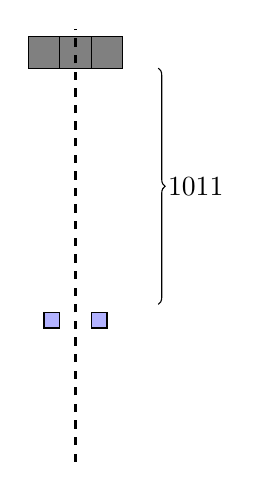
\begin{tikzpicture}
        \gokart{0}{0}{0}
    
        % Wall (three cubes)
        \draw[fill=gray] (-0.6,3) rectangle (-0.2,3.4);
        \draw[fill=gray] (-0.2,3) rectangle (0.2,3.4);
        \draw[fill=gray] (0.2,3) rectangle (0.6,3.4);
    
        % Dashed line from go-kart to wall (center axis)
        \draw[dashed, thick] (0,-2) -- (0,3.5);
    
        % Range brace annotation
        \draw [decorate, decoration = {brace, raise=10pt}] (0.7,3) -- (0.7, 0) node[pos=0.5,right=10pt,black]{\SIrange{10}{11}{\meter}};

        % Enlarged Radar sensor boxes
        \draw[fill=blue!30] (-0.4,-0.3) rectangle (-0.2,-0.1);
        \draw[fill=blue!30] (0.2,-0.3) rectangle (0.4,-0.1);
    \end{tikzpicture}
    \caption{Test scenario with dual front-mounted mmWave radar sensors.  
    This setup served as the baseline validation environment before moving to more complex scenarios.}
    \label{fig:test_scenario}
\end{figure}

The dual-radar arrangement increases point density and stability compared to single-radar approaches, aligning with multimodal strategies for robust state estimation \cite{Multimodal_Offroad,HighSpeed_Estimation}.  
By fusing radial speed measurements obtained from Doppler with rotational information from the IMU, the proposed system is designed to remain resilient even in scenarios where LiDAR- or camera-based odometry would degrade.  
Each radar stream is first processed independently and then merged into a combined representation before feeding into the odometry pipeline.  

\subsubsection{Sub-Tasks}

The research objective, together with the constraints of using a dual-radar sensor, implied several practical sub-tasks:  
\begin{itemize}
    \item Designing a modular pipeline to acquire and decode synchronized radar data from both sensors.  
    \item Investigating suitable sensor configurations to balance field of view, chirp bandwidth, update rate, and detection density.  
    \item Developing suitable mechanical mounts and selecting optimal sensor placement to ensure stability and maximize coverage.  
    \item Applying RANSAC filtering on Doppler velocities to reject dynamic points and outliers.  
    \item Implementing clustering methods to structure radar detections and isolate relevant features.  
    \item Optimizing the raw radar point cloud using additional information provided by the sensor itself (e.g., SNR, RCS, or range validity) to improve reliability before odometry processing.  
    \item Integrating Doppler velocity information into the odometry estimation process.  
    \item Employing submap aggregation to mitigate sparsity and improve stability.  
    \item Performing ICP alignment between submaps aggregated from both sensors to mitigate sparsity and noise.  
    \item Evaluating the influence of the dual-sensor arrangement on odometry accuracy and robustness.  
    \item Validating the complete system on real-world driving scenarios.  
\end{itemize}

As each sub-task builds upon the results of the previous one, the work followed an iterative and modular development approach, enabling gradual integration and continuous evaluation of the proposed system.  
The following sections detail the hardware design, pipeline methodology, and experimental validation.  

\begin{comment}
    Here we start the System Hardware section
    System Hardware
    - Sensors (radar, IMU, webcam).
    - Mechanical integration (3D printed mounts, placement, calibration).
    - Chirp configuration & radar setup.
    * Keep at a descriptive/theoretical level (role of each hardware element in methodology). 

\end{comment}

